%********************************************************************************
% Title: Smart Elasticity leveraging Reinforcement Learning in Kubernetes
%
% Author: Giacomo Marciani <mgiacomo@amazon.com>
%
% Institution: Department of Civil Engineering and Computer Science Engineering,
% University of Rome Tor Vergata, Italy
%
% Style: ACM ART SIGCONFS (based on ACM Large v1.7)
%*******************************************************************************

\documentclass[12pt,oneside,vi]{mitthesis}
\usepackage{lgrind}
\usepackage{cmap}
\usepackage[T1]{fontenc}
\usepackage{graphicx}
\usepackage{array}
\usepackage{lscape}
\usepackage[ruled,noend,noline,linesnumbered]{algorithm2e}
\usepackage{lipsum}
\usepackage{amsmath}
\usepackage{amsthm}
\usepackage{amssymb}
\usepackage{hyperref}
\usepackage{listings}

\pagestyle{plain}

\graphicspath{ {./fig/} {./fig/plot/} }

\newtheorem{theorem}{Theorem}

\setlength\extrarowheight{5pt}

\begin{document}

\title{Heuristics for elastic container orchestration}

\author{Giacomo Marciani}

\department{Department of Civil and Computer Science Engineering}

\degree{Master of Science in Computer Science Engineering and Data Science}

\degreemonth{May}

\degreeyear{2018}

\thesisdate{May 18, 2018}
 
\copyrightnoticetext{\copyright Giacomo Marciani, 2018.}

\supervisor{Valeria Cardellini}{Associate Professor}

\supervisor{Matteo Nardelli}{PhD Student}

%\chairman{Arthur C. Smith}{Chairman, Department Committee on Graduate Theses}

%\maketitle

\cleardoublepage
\pagestyle{empty}
\setcounter{savepage}{\thepage}

\begin{abstractpage}
\begin{abstract}
We prove the semi-decidability of the problem of saying whether or not a context-free grammar generates a regular language.
We introduce the notion of context-free grammar in Marciani Normal Form.
We prove that a context-free grammar in Marciani Normal Form always generates a regular language.
\end{abstract}

\end{abstractpage}

\cleardoublepage

%% acknowledgments.tex

% From mitthesis package
% Version: 1.01, 2023/10/16
% Documentation: https://ctan.org/pkg/mitthesis


\chapter*{Acknowledgments}
\addcontentsline{toc}{chapter}{Acknowledgments}

I would like to express my deepest gratitude to all those who have supported me throughout this research and my overall course of study.

First and foremost, I would like to thank with all my heart my beloved wife and my parents for always motivating me to conclude my thesis and believing in me in good and bad times.

I thank my sons Edoardo, Arianna and Vittorio because they fill my life with love and their birth has been the strongest motivation to complete my studies.

I thank my grandfather for passing on my passion for computer science to me since I was a child.

A special thanks goes to my friends and colleagues, Antonella, Debora, Gianluca, Giorgio and Michele: we shared joys and sorrows during my university journey and they motivated me to complete my thesis every time we met.

I'd like to thank my advisor, Prof. Salvatore Filippone, whose expertise, encouragement, and insightful feedback were invaluable in shaping this thesis.

I thank Prof. Valeria Cardellini for passing on to me the passion for distributed systems, that shaped my entire career.

Last but not least, I thank my amazing company Amazon Web Services for betting on me even before I finished my studies.


\pagestyle{plain}
\include{sec/contents}
\section{Introduction}
\label{sec:introduction}

In \Cref{sec:definitions}, we give some preliminary definitions about language
equations and the regularity problem.
In particular, we introduce the class of bilateral-linear language equations,
the pseudo-regular partition of productions and the looking forward property.

In \Cref{sec:marciani-rule}, we state and prove Marciani's Rule, which exposes
a method to solve the bilateral-linear language equations.

In \Cref{sec:marciani-normal-form}, we define the Marciani Normal Form, and we
prove that a context-free grammar in such a form always generates a regular
language.

In \Cref{sec:semi-decidability}, we prove the semi-decidability and the
undecidability of the context-free regularity problem, by the application of the 
previous results.

In \Cref{sec:examples}, we give some applicative examples of the Marciani's Rule
and the Marciani Normal Form.

\chapter{Smart Elasticity}
\label{chp:smart-elasticity}


% %
% HEADER
% %
The smart elasticity is the ability of a system to dynamically auto-scale resources according to scaling policies determined with machine learning techniques.
%
The smart elasticity service hence provides a resource manager, e.g. a container orchestrator, with the ability to learn the best replication degree for its resources, e.g. deployed containers, with respect to the current cluster state.
%
In this work we propose to implement smart elasticity for Kubernetes leveraging reinforcement learning, that is the most famous technique of unsupervised machine learning.
%
In particular, we focus on $\mathcal{Q}$-Learning, which is the most widely studied reinforcement learning algorithm.
%
In this Chapter we show the adopted reinforcement learning model, the pseudocode of the learning algorithm that realizes it and the implementation of the overall service.

%
%First, we exlain how the general Q-Learning algorithm can be adapted to achieve smart elasticity. In particulr, we show the pseudocode that implements the algorithm.
%
%Then, we show how the smart elasticity service has been implemented in the Kubernetes environment. 
%In particular, we show the reference architecture, component interactions and the REST interfaces.


% %
% ELASTICITY LEVERAGING Q-LEARNING
% %
\section{Elasticity leveraging $\mathcal{Q}$-Learning}
\label{sec:smart-elasticity-elasticity-leveraging-q-learning}

A reinforcement learning algorithm can be used to learn the best scaling policy to adopt in response to cluster state changes without any past knowledge.
%
In this work, we propose an approach that makes use of the $\mathcal{Q}$-Learning algorithm, described in Chapter \ref{chp:reinforcement-learning}.
%
A general $\mathcal{Q}$-Learning algorithm relies on a reinforcement learning model that requires the definition of the following spaces, functions and parameters:

\begin{itemize}
	
	\item State Space $\mathcal{S}$ where each state $s\in\mathcal{S}$ is a cluster state.
	
	\item Action Space $\mathcal{A}$ where each action $a\in\mathcal{A}$ is a scaling action.
	
	\item Quality Function $\mathcal{Q}:\mathcal{S}\times\mathcal{A}\rightarrow\Re$ where the value $q_{s_{t},a_{t}}=\mathcal{Q}(s_{t},a_{t})$ is the quality of performing the action $a_{t}$ in the state $s_{t}$ at time $t$.
	%
	Notice that, since Q-Learning is an iterative algorithm that updates $\mathcal{Q}$, this function requires an initialization setting $\mathcal{Q}_{0}$.
	
	\item Rewarding Function $\mathcal{R}:\mathcal{S}\rightarrow\Re$ where the value $r_{t}=\mathcal{R}(s_{t})$ is the rewarding achieved for the state $s_{t}$.
	
	\item Learning Rate $\alpha\in (0,1]$ that trades off the importance of sooner versus later quality values 
	
	\item Discount Factor $\gamma\in [0,1]$ that trades off the importance of sooner versus later rewards.
\end{itemize}

These items encapsulate the peculiarities of the domain where the algorithm is applied and are used by the Agent to determine the optimality of an action in a state, according to the following update:

\begin{equation}
	\label{eqn:smart-elasticity-reinforcement-learning-update}
	\mathcal{Q}(s_{t},a_{t}) \leftarrow (1-\alpha) \cdot \mathcal{Q}(s_{t},a_{t}) + \alpha \cdot (r_{t} + \gamma \cdot \max_{a}(\mathcal{Q}(s_{t+1},a_{t}))
\end{equation}

In the following, we show and motivate our choice for the aforementioned parameters in the context of smart elasticity.


\subsection{State Space}
\label{sec:smart-elasticity-elasticity-leveraging-q-learning-state-space}

INSERT HERE DESCRIPTION OF THE STATE SPACE (ITERATE WITH PROF).


\subsection{Action Space}
\label{sec:smart-elasticity-elasticity-leveraging-q-learning-action-space}

INSERT HERE THE DESCRIPTION AND MOTIVATIONS OF THE CHOOSEN ACTION SPACE (ITERATE WITH PROF).


\subsection{Quality Function}
\label{sec:smart-elasticity-elasticity-leveraging-q-learning-quality-function}

INSERT HERE THE DESCRIPTION AND MOTIVATIONS OF THE CHOOSEN QUALITY FUNCTION (ITERATE WITH PROF).


\subsection{Rewarding Function}
\label{sec:smart-elasticity-elasticity-leveraging-q-learning-rewarding-function}

INSERT HERE THE DESCRIPTION AND MOTIVATIONS OF THE CHOOSEN REWARDING FUNCTION (ITERATE WITH PROF).


\subsection{Learning Rate}
\label{sec:smart-elasticity-elasticity-leveraging-q-learning-learning-rate}

INSERT HERE THE DESCRIPTION AND MOTIVATIONS OF THE CHOOSEN LEARNING RATE (ITERATE WITH PROF).


\subsection{Discount Factor}
\label{sec:smart-elasticity-elasticity-leveraging-q-learning-discount-factor}

INSERT HERE THE DESCRIPTION AND MOTIVATIONS OF THE CHOOSEN DISCOUNT FACTOR (ITERATE WITH PROF).


% %
% ALGORITHM
% %
\section{Algorithm}
\label{sec:smart-elasticity-algorithm}

INSERT HERE A DETAILED DESCRIPTION OF THE PSEUDOCODE IN ALGORITHM \ref{alg:smart-elasticity-algorithm}.

\begin{algorithm}[t]
	\label{alg:smart-elasticity-algorithm}
	\SetKwProg{Fn}{Function}{}{}  
	
	\Fn{foo (bar)} {
		$print "Hello World"$ \\
	}
	\caption{Pseudocode of the \texttt{SmartElasticity} algorithm.}
\end{algorithm}


% %
% IMPLEMENTATION
% %
\section{Implementation}
\label{sec:smart-elasticity-implementation}

The smart elasticity service is realized by the following four main components, interacting via REST interfaces.
%
In Figure \ref{fig:smart-elasticity-architecture} we show the high-level reference architecture for the smart elasticity service, represented as a UML component diagram.

\begin{itemize}
	
	\item \texttt{ClusterMonitor} collects cluster performance metrics focused on CPU, Memory and Network utilization in a per-node and/or per-container basis. 
	%
	These metrics can be queried via a REST interface.
	%
	In a usual Kubernetes cluster, this component is realized by the Heapster master.
	
	\item \texttt{Orchestrator} responsible for containers orchestration. 
	%
	In particular, it deployes containers and dynamically scales them in/out accordingly with the scaling actions provided by the \texttt{ScalerAI}.
	%
	It pulls \texttt{ScalerAI} at fixed time interval to retrieve the scaling action to perform with respect to the current cluster state. 
	%
	Since the smart elasticity service can be provided to distinct cluster contexts, a token is required to identify the context during REST inetractions.
	%
	In a usual Kubernetes cluster, this component is realized by the Kubernetes leading master.
	
	\item \texttt{ScalerAI} responsible for the smart elasticity service.
	%
	In particular it determines the best scaling action with respect to the current cluster state accordingly to the adopted reinforcement learning technique. 
	%
	It exposes a REST interface through which the \texttt{Orchestrator} can ask for scaling actions.
	%
	When this component is asked to produce a new scaling action, the \texttt{StateManager} collects metrics from the \texttt{ClusterMonitor} and aggregates them into a new \texttt{ClusterState}, representing the current cluster state.
	%
	Notice that the cluster state should aggregate all those metrics required to compute the current state, quality and rewarding function.
	%
	The latter are then used by the \texttt{RLAgent} to execute the reinforcement learning algorithm to produce the new \texttt{ScalingAction}.
	%
	The \texttt{RLAgent} reads/writes all data required by the RL algorithm from/to the \texttt{RLDataManager}, that is responsible to store data into the \texttt{RLRepository}.
	%
	Notice that both the \texttt{StateManager}, \texttt{RLDataManager} and \texttt{RLAgent} are configured by external files.
	%
	The \texttt{StateConfig} provides the \texttt{StateManager} with the addresses of the REST interfaces to interact with the \texttt{ClusterMonitor}.
	%
	The \texttt{RepositoryConfig} provides the \texttt{RLDataManager} with the addresses of the REST interfaces to interact with the \texttt{RLRepository}.
	%
	The \texttt{LearningConfig} provides the \texttt{RLAgent} with set of parameters required by the reinforcement learning algorithm.
	
	\item \texttt{RLRepository} a data store reponsible for storing data required by \texttt{RLAgent} for the execution of the reinforcement learning algorithm, e.g. parameters and reinforcement learning matrices.
	
\end{itemize}

From a technological point of view, the \texttt{ScalerAI} has been implemented as a Spring-based REST service, that is a de-facto standard solution for Java enterprise web applications; while the \texttt{RLRepository} has been implemented as a MongoDB datastore, which is a de-facto standard technology for NoSQL document-based datastore. 

Let us now focus on the interactions flow that realizes the smart elastic auto-scaling.
%
In Figure \ref{fig:smart-elasticity-sequence-diagram} we show the flow of interactions between components of the auto-scaling service, represented as a UML sequence diagram.

\begin{enumerate}
	
	\item the \texttt{Orchestrator} asks \texttt{ScalerAI} to compute a new scaling action. The request is submitted to the \texttt{ScalerAIController}, which is the \texttt{ScalerAI} entry-point.
	
	\item the \texttt{ScalerAIController} retrieves the current cluster state from the \texttt{StateManager}. The custer state encapsulates the cluster performance metrics of interest, gathered from the \texttt{ClusterMonitor}.
	
	\item the \texttt{ScalerAIController} asks the \texttt{RLAgent} to compute a new scaling action with respect to the current cluster state.
	
	\item the \texttt{RLAgent} (i) computes the current state $s\in\mathcal{S}$ and, concurrently, (ii) retrieves reinforcement learning data from the \texttt{RLDataManager}, which collects it from the \texttt{RLRepository}.
	
	\item the \texttt{RLAgent} uses he gathered state and data to compute sequentially (i) the rewarding function, (ii) the quality function and (iii) the action.
	
	\item the \texttt{RLAgent} concurrently (i) saves new function values to the \texttt{RLRepository} via the \texttt{RLRepositoryManager} and (ii) encapsulates the computed action into a new \texttt{ScalingAction} returned to the \texttt{ScalerAIController}.
	
	\item the \texttt{ScalerAIController} returns the new scaling action to the \texttt{Orchestrator}.
	
	\item the \texttt{Orchestrator} apply the scaling action.
	
\end{enumerate}

%\clearpage
%\vfill
\begin{figure}	
	\label{fig:smart-elasticity-architecture}
	\centering
	\includegraphics[width=.85\columnwidth]{smart-elasticity-architecture}
	\caption{The architecture.}
\end{figure}
%\vfill
\clearpage
\vfill
\begin{landscape}
	\begin{figure}	
		\label{fig:smart-elasticity-sequence-diagram}
		\centering
		\includegraphics[width=.85\columnwidth]{smart-elasticity-sequence-diagram}
		\caption{The auto-scaling activity.}
	\end{figure}
\end{landscape}
\vfill
\clearpage


% %
% REST INTERFACES
% %
\subsection{REST Interfaces}
\label{sec:smart-elasticity-implementation-rest-interfaces}

In this section we detail the REST API exposed by the \texttt{ScalerAI} to manage learning contexts and provide the \texttt{Orchestrator} with the \texttt{ScalingAction}. 
%
Furthermore we detail the REST calls executed by ScalerAI on ClusterMonitor to gather the performance metrics.

\begin{table}
	\label{tbl:smart-elasticity-rest-scalerai}
	\centering
	\begin{tabular}{| m{1.5cm} | m{3cm} | m{3cm} | m{8cm} | }\hline
		
		\textbf{Method} & \textbf{Resource} & \textbf{Params} & \textbf{Description} \\\hline

		\texttt{GET}	& scaling-action  & api-token & Retrieves a new scaling action. \\\hline

		\texttt{GET}    & context         & api-token & Retrieves the learning context. \\\hline
		
		\texttt{PATCH}  & context         & api-token, learningParameters & Modifies the learning context. \\\hline
		
	\end{tabular}
	\caption{The REST interface exposed by \texttt{ScalerAI}.}
\end{table}

\begin{table}
	\label{tbl:smart-elasticity-rest-cluster-monitor}
	\centering
	\begin{tabular}{| m{1.5cm} | m{3cm} | m{3cm} | m{8cm} | }\hline
		
		\textbf{Method} & \textbf{Resource} & \textbf{Params} & \textbf{Description} \\\hline
		
		\texttt{???}	& ???               & ???             & ??? \\\hline
		
		\texttt{???}	& ???               & ???             & ??? \\\hline
				
		\texttt{???}	& ???               & ???             & ??? \\\hline
		
	\end{tabular}
	\caption{The REST interface of interest exposed by Heaster.}
\end{table}
\chapter{Reinforcement Learning}
\label{chp:reinforcement-learning}


% %
% HEADER
% %
\lipsum[1]

Reinforcement
Learning (RL) refers to a collection of trial-and-error methods by which an agent
can learn to make good decisions through a sequence of interactions with a
system or environment


% %
% DEFINITIONS
% %
\section{Definitions}
\label{sec:reinforcement-learning-definitions}

One
of the challenges that arise in reinforcement learning is the trade-off between
exploration and exploitation. To maximize the obtained reward, a RL agent
must prefer actions that it has tried in the past and found to be effective in
producing reward (exploitation). However, in order to discover such actions, it
has to try actions that it has not selected before (exploration). The dilemma
is that neither exploration nor exploitation can be pursued exclusively without
failing at the task. The agent must try a variety of actions and progressively
favor those that appear to be best [12]. To the best of our knowledge, only one
work [5] has so far exploited RL techniques to drive the auto-scaling decisions in
DSP systems. Heinze et al. [5] propose a simple RL approach that learns from
experience when to acquire and release computing nodes so to efficiently process
the incoming workload. The per-operator auto-scaler populates a lookup table
that associates the utilization of the node on which the operator is executed with
the action to perform (i.e., scale in, scale out, or do nothing). The adaptation
goal is to keep the system utilization within a specific range; the SARSA learning
algorithm [12] is used to update the lookup table.
A larger number of works has exploited RL techniques to drive elasticity in
the Cloud computing context, as surveyed in [9]. Most of them use the simple Q-
learning RL algorithm (described in Sec. 5), which suffers from slow convergence,
as we also show in Section 6. Tesauro et al. [13] observe that RL approaches
can suffer from poor scalability in systems with a large state space, because
the lookup table has to store a separate value for every possible state-action
pair. Moreover, the performance obtained during the on-line training may be
unacceptably poor, due to the absence of domain knowledge or good heuristics.
To overcome these issues, they combine RL with a model of the system, defined
using queuing theory, which computes the initial deployment decisions and drives
the exploration actions. They use the SARSA learning algorithm, which however
suffers from slow convergence as Q-learning.

The goal of the Operator Manager is to take scaling decisions as to minimize
a long-term cost function which accounts for the operator downtime and for the
monetary cost to run the operator. The latter comprises: (i) the cost for running
the number of instances during the next time slot, and (ii) possibly a penalty
in case of SLA violation. In particular, we consider a constraint on the operator
response time, so that a penalty is paid every time the response time exceeds a
given threshold T SLA.

Since decisions are taken periodically, we consider a slotted time system with
fixed-length time intervals of length ∆t, with the i-th time slot corresponding
to the time interval [i∆t, (i + 1)∆t] (see Fig. 2). We denote by k i the number
of parallel instances at the beginning of slot i, and by λ i the average tuple rate
during slot i − 1 (the previous slot). At the beginning of slot i the Operator-
Manager makes the decision a i on whether modify or keep the current instance
configuration.


% %
% Q-LEARNING
% %
\section{Q Learning}
\label{sec:reinforcement-learning-q-learning}

It has been proven that, independently of the policy
being followed and the initial values assigned to Q, the learned action-value
function converges with probability 1 to Q ∗ \cite{watkins1992q}, under the condition that every
state-action pair continues to be sampled as i → ∞.


% %
% PDS-LEARNING
% %
\section{PDS Learning}
\label{reinforcement-learning-pds-learning}

In order to integrate the partial knowledge of the system into a learning
algorithm, we rely on the post-decision state (PDS) concept, exploiting the gen-
eralized definition given in [10]. A PDS (also known as afterstate) describes the
state of the system after the known dynamics take place, but before the unknown
dynamics take place. 

where s  ̃ i fully reflects the consequences of the action a i , and the next state s i+1
incorporates the unknown system dynamics (i.e., the input rate variation).

We exploit the PDS concept to design a learning algorithm that aims at
finding an optimal policy in less time than Q-Learning. To this end, we adapt
the algorithm proposed in [10] to our problem. We integrate that solution into
the generic Algorithm 1 by extending the update phase. In particular, the Q
function has only to deal with the known system dynamics, since the unknown
parts are hidden by the PDS, for which we introduce a PDS value function V  ̃
that is updated along with Q

It is worth noting that, since the unknown system dynamics do not depend on
the selected action, randomized exploration is not required any more, and a
greedy policy can be followed during the learning phase.

% %
% FULL BACKUP LEARNING
% %
\section{FBMB Learning}
\label{reinforcement-learning-fbmb-learning}

\lipsum[1]
\chapter{Kubernetes}
\label{chp:kubernetes}

Kubernetes is a production-grade open-source container orchestrator, originally designed by Google.
%
It was soon established as a de-facto standard for automated management, deployment, scaling and CI/CD of containerized micro-service applications in large clusters.
%
%
%Basically, it runs containers on a cluster abstracted as a transparent pool of resources, so as to optimize resources usage and to scale and update containers with no down-time.
%
We choose Kubernetes as the container orchestrator on which to conduct our experiments because 
(i) it is an industrial standard,
(ii) it is portable, extensible and autonomic,
(iii) it is designed for long-running micro-services applications,
(iv) it is based on a innovative deployment schema (Pods)
(iv) it is open-source,
(vi) it is well documented,
(vii) it is supported by an active community.

In this Chapter, we give an overview of Kubernetes as our reference platform to implement and experiment smart elasticity.
%
In particular, we introduce it with a bit of its history, then focus on its main features, architecture, objects and the way it provides elasticity.


% %
% HISTORY
% %
\section{History}
\label{sec:kuberetes-history}
The name Kubernetes originates from the Greek word $\kappa\upsilon\beta\epsilon\rho\nu\epsilon\tau\epsilon\sigma$, that means \textit{helmsman} and is also the etymological root of the term cybernetic\footnote{term coined in 1948 by U.S. mathematician Norbert Wiener (\cite{masani2012norbert}).}.
%
Kubernetes is often refer to as \textit{K8s}, derived by replacing the 8 letters "ubernete" with "8".

Kubernetes was originally designed by Google as the open-source declination of Omega (\cite{burns2016borg}), that is the closed-source containers orchestrator internally used by Google to manage its two billions running containers (\cite{schwarzkopf2013omega}).
%
Kubernetes builds upon over a decade of experience that Google has with running production workloads at scale, combined with best-of-breed ideas and practices from the community (\cite{verma2015large}).
%
The first release was announced on June 2014 with a blog post on \cite{google-announces-kubernetes} and became soon available to the public through the Google Container Engine (\cite{google-container-engine-web}).
%
In 2015, it was donated to the Cloud Native Computing Foundation (\cite{techcrunch-kubernetes-cncf}), a department of the Linux Foundation (\cite{linux-foundation-web}) (the world's largest open source non-profit organization) founded by world's leading tech companies such as Google, IBM and VMWare to promote containers (\cite{zdnet-cncf}).
%
The explosion in popularity of containerization has heavily impacted the development and adoption of Kubernetes.


% %
% FEATURES
% %
\section{Features}
\label{Sec:features}

Kubernetes coordinates a highly available cluster of VMs or physical machines to work together as a single unit. 
%
It provides abstractions that allow to deploy containerized applications to a cluster without hard-wiring them to individual nodes.
%
Hence it realizes a truly \textit{container-centric environment}, opposed to the traditional host-centric infrastructure, which provides the full advantages and benefits inherent to containers.

Kubernetes allows the cluster manager to effectively automate applications delivery to customers by 
(i) deploying containerized applications quickly and predictably,
(ii) scaling applications on the fly,
(iii) rolling out new features with no downtime and
(iv) optimizing resource usage by limiting it to required resources only.

%Kubernetes is 
%(i) \textit{portable}, as it supports both public, private, hybrid and multi-cloud
%(ii) \textit{general purpose}, as it supports both stateless/stateful, micro-service/monoliths and service/batch applications,
%(iii) \textit{extensible}, as it is modular, pluggable, hookable and composable, and
%(iv) \textit{autonomic}, as it provides self-healing functionalities, such as auto-restart, auto-placement and auto-scaling.

The Kubernetes project has been always committed to the following design pillars:

\begin{itemize}
	
	\item \textbf{Portability:} supports both public cloud, private cloud, bare metal and laptop with consistent behavior so that applications and tools are portable throughout the ecosystem.
	
	\item \textbf{Generality:} it is agnostic to applications, as it runs applications that are both stateless and stateful, microservices and monoliths, services and batch, and so on.
	
	\item \textbf{Meet users partway} although it focuses on deployment and management of microservices and cloud-native applications, it provides some mechanisms to facilitate migration of monolithic and legacy applications.
	
	\item \textbf{Flexibility} its functionalities can be consumed a la carte and (in most cases) Kubernetes does not prevent from using custom solutions in lieu of built-in functionalities.
	
	\item \textbf{Extensibility} Kubernetes enables you to integrate it into your environment and to add the additional capabilities you need, by exposing the same interfaces used by built-in functionalities.
	
	\item \textbf{Automation} it dramatically reduce the burden of manual operations. It supports both declarative and imperative control to support higher-level orchestration and automation. The declarative approach is key to the system’s autonomic capabilities.
	
	\item \textbf{CI/CD} users expect applications to be available all the time and developers are expected to deploy new versions frequently.
	%
	Kubernetes provides a mechanism to rool-out/roll-back containers with zero downtime by incrementally updating application instances with new ones and load-balancing the traffic only to available Pods during the update.
	
	\item \textbf{Advance the state of the art} although it intends to support non-cloud-native applications, it aims to drive and advance the cloud-native and DevOps state of the art.
	
\end{itemize}



% %
% ARCHITECTURE
% %
\section{Architecture}
\label{sec:kubernetes-architecture}

Kubernetes follows a master-worker distributed architecture, as depicted in Figure \ref{fig:kubernetes-architecture}.
%
A production Kubernetes cluster should have a minimum of three nodes, one serving as a Kubernetes Master and two serving as Kubernetes Workers.

The \textbf{Kubernetes Master} is responsible for managing the cluster, coordinating all activities, such as scheduling applications, defining and maintaining their desired state, scaling them, and rolling out new updates.
%
The master controls each node so that it is rare to interact with workers directly.
%
The master can be run on a single node, or can be replicated in order to support high-availability clusters.
%
The Master executes the following processes:
%
\begin{itemize}
	
	\item \textbf{API Server:} a web server that exposes a RESTful API to let the user interact with the master to manage the whole cluster.
	%
	Basically, it provides the front-end to the cluster’s shared state through which all other components interact with.
	%
	For example, it allows the user to configure the cluster, check up its state, create, update and delete Kubernetes Objects.
	%
	The \texttt{kubectl} utility is the most convenient way to instruct the server because it encapsulates REST calls into simple and intuitive terminal commands.
	
	\item \textbf{Controller Manager:} a daemon that coordinates all core controllers.
	%
	Each controller watches a portion of the shared state of the cluster and makes changes to drive the actual state towards the desired state.
	%
	These functions have been split into separate components to make them more easily replaceable and extendable.	
	
	\item \textbf{Scheduler:} a policy-rich and topology-aware daemon that determines how to schedule and place containerized applications on Workers.
	%
	To determine the best fit it takes into account a lot of factors, such as resources utilization, quality of service requirements, hardware/software/policy constraints, affinity and anti-affinity specifications, data locality and son on.
	%
	%Kubernetes supports user-provided schedulers and multiple concurrent cluster schedulers, using the shared-state approach pioneered by Omega.
	
	\item \textbf{ETCD:} a distributed reliable key-value database, used to store cluster's state and configurations\footnote{the name \textit{ETCD} is inspired by the Unix system folder \textit{etc}, used to store system configurations, to which the letter \textit{d} has been added with the meaning of \textit{distributed}.} in JSON or Protobuf format.
	%
	It provides a way to store configuration data reliably and to coordinate components by meant of cluster's state changes and can be inspected using the \textit{etcdctl} tool.
	
\end{itemize}

A \textbf{Kubernetes Worker} is responsible for the execution of Pods and to notify local resource state to the Master.
%
Each Worker executes the following processes:
%
\begin{itemize}
	
	\item \textbf{Kubelet:} the primary agent responsible for communication between the Kubernetes Master and the Node and the management of all Pods scheduled on its Node.
	%
	The kubelet works in terms of a \textit{PodSpec}, that is a YAML or JSON that describes a Pod.
	%
	The kubelet takes a set of PodSpecs that are provided through various mechanisms (primarily through the apiserver) and ensures that the containers described in those PodSpecs are running and healthy.
	
	\item \textbf{Container Runtime:} a runtime environment responsible for managing images and running containers.
	%
	Future versions will be provided with a Container Runtime Interface to decouple scheduling operations from the underlying control of containers in order to facilitate pluggability of the container runtime.
	%
	The current version supports Docker (\cite{docker-web}), Rkt (\cite{rkt-web}), Cri-o (\cite{crio-web}), and Frakti (\cite{frakti-web}).
	
	\item \textbf{Proxy:} a daemon responsible for routing requests submitted to Service external IP to the internal virtual IP of the attached back-ends, in a highly-available and load balanced fashion.
	%
	When a user creates a new Service, new rules are added to this component.
	
	\item \textbf{cAdvisor:} a daemon that collects, aggregates and exports performance metrics about containers running on the Node.
	%
	It natively supports Docker containers but future versions are going to support any other container type out of the box.
	
\end{itemize}

Furthermore, a Kubernetes cluster is provided with \textbf{Cluster Add-Ons}, that are built-in Deployments and Services considered an inherent part of a Kubernetes cluster.
%
The most notable addons are \textit{GUI}, providing a convenient web interface to interact with the cluster, and \textit{Heapster}, providing monitoring service about performance statistics for the whole cluster.
%
For a complete list of such add-ons, we refer the reader to \cite{kubernetes-web}.

The Kubernetes architecture is often partitioned into
(i) the \textbf{Control Plane}, constituted by the Kubernetes Master and Kubelet, responsible to make the cluster’s current state match the desired state.
(ii) the \textbf{Execution Plane}, constitute by Container Runtime, Proxy, cAdvisor and add.ons, responsible for the real execution of containers.

\begin{figure}	
	\label{fig:kubernetes-cluster}
	\centering
	\includegraphics[width=.7\columnwidth]{kubernetes-cluster}
	\caption{Kubernetes cluster.}
\end{figure}

\begin{figure}	
	\label{fig:kubernetes-architecture}
	\centering
	\includegraphics[width=.7\columnwidth]{kubernetes-architecture}
	\caption{Kubernetes architecture.}
\end{figure}


\section{Objects}
\label{sec:kubernetes-objects}
Kubernetes provides some abstractions to represent and manage the state of the cluster.
%
These abstractions are called \textit{Kubernetes Objects} (or simply Objects, for short) and are persistent entities within the Kubernetes system, thus representing the core API building blocks.
%
Each Kubernetes Object characterizes the desired cluster's state, that is why it is sometimes refer to as a "record of intent".
%
Objects are managed, i.e. created updated and deleted, by submitting requests to the Kubernetes REST API.

The main abstractions, at least the ones related to our work, are \textit{Deployment}, \textit{Pod}, \textit{Service} and \textit{HorizontalPodAutoscaler}.
%
We refer the reader to \cite{kubernetes-web} for a complete description of all objects.

A \textbf{Deployment} defines the desired state for an application in a declarative fashion.
%
It defines the state in terms of 
(i) composing containers 
(ii) number of replicas
(iii) constraints of resource utilization
%
The creation of a new Deployment is the creation of a new invariant to satisfy.

A \textbf{Pod} is the smallest deployable unit of computing that can be created and managed in Kubernetes, serving as a unit of deployment, horizontal scaling, and replication.
%
A Pod is a group of one or more containers that are co-scheduled on the same node together with a specification defining how to run them.
%
Containers in a Pod share the same storage (volumes) and network (IP address, port space); furthermore they can easily communicate via IPC primitives.
%
This is why containers that need to work together are usually added to the same Pod.
%
A Pod should be viewed as a cohesive unit of service and it can be made of 
(i) a single container, where a Pod is a simple wrapper around a container or 
(ii) a group of tightly coupled containers forming a single instance of a composite application.
%
For example a Pod can be used to host vertically integrated application stacks, such as LAMP.
%
Like well-designed containers following the micro-services model, well-designed pods should be \textit{focused}, \textit{stateless}, and \textit{concurrent}, as Kubernetes assumes that pods can be deleted, created, and replicated at will.
%
Pod abstraction is convenient because it realizes decoupling of software dependencies thus making easier and more effective the general management and the CI/CD automation.
%
%A Pod's lifecycle is made of the following phases:
%
%\begin{itemize}
%	\item \textbf{Pending:} The API Server has created a pod resource and stored it in etcd, but the pod has not been scheduled yet, nor have container images been pulled from the registry.
%	\item \textbf{Running:} The pod has been scheduled to a node and all containers have been created by the kubelet.
%	\item \textbf{Succeeded:} All containers in the pod have terminated successfully and will not be restarted.
%	\item \textbf{Failed:} All containers in the pod have terminated. At least one container has terminated in failure.
%	\item \textbf{Unknown:} The API Server was unable to query the state of the pod, typically due to an error in communicating with the kubelet.
%\end{itemize}
%
%When you do a kubectl get pod, note that the STATUS column might show a different message than the above five messages, such as Init:0/1 or CrashLoopBackOff. This is due to the fact that the phase is only part of the overall status of a pod.
%
%Not shown in the diagram, before anything else, the infra container is launched establishing namespaces the other containers join.
%The first user-defined container launching is the init container which you can use for pod-wide initialization.
%Next, the main container and the post-start hook launch at the same time, in our case after 4 seconds. You define hooks on a per-container basis.
%Then, at second 7, the liveness and readiness probes kick in, again on a per-container basis.
%At second 11, when the pod is killed, the pre-stop hook is executed and finally, the main container is killed, after a grace period. Note that the actual pod termination is a bit more complicated.
%
%The livenessProbe is used by the kubelet to determine if and when to re-start a container and by a deployment to decide if a rolling update is successful.
%
%The readinessProbe is used by a service to determine if a pod should receive traffic.
%
%\begin{figure}	
%	\label{fig:kubernetes-pod-lifecycle}
%	\centering
%	\includegraphics[width=.7\columnwidth]{kubernetes-pod-lifecycle}
%	\caption{Kubernetes Pod lifecycle.}
%\end{figure}

A \textbf{Service} defines single long-running access-point for a logical set of Pods.
%
It allows
(i) load-balanced exposure to external traffic (although each Pod has a unique IP address, those IPs are not exposed outside the cluster without a Service),
(ii) routing across dependent Pods (entities do not communicate with a specific Pod, but with a Service)
(iii) loose coupling between dependent Pods (distinct application services are managed by distinct Service abstractions).
(vi) auto-scaling with no down-time, as the Service ensures lets new replicas dynamically join/exit the set of Pods.

Each object instance can be associated with a collection of \textit{labels}, that are key/value pairs metadata that can be used to classify and filter objects.
%
For example, a Service can be defined to expose only Pods with a specific label, so as to automatically join those Pods once created.

\begin{figure}	
	\label{fig:kubernetes-services}
	\centering
	\includegraphics[width=.7\columnwidth]{kubernetes-services}
	\caption{Kubernetes Service deployment.}
\end{figure}

\begin{figure}	
	\label{fig:kubernetes-horizontal-pod-autoscaler}
	\centering
	\includegraphics[width=.7\columnwidth]{kubernetes-horizontal-pod-autoscaler}
	\caption{Kubernetes Horizontal Pod Auto-scaler.}
\end{figure}

A \textbf{HorizontalPodAutoscaler} defines the range of resources utilization that each Pod should work in, inducing horizontal scaling actions to satisfy these bounds.
%
We refer the reader to Section \ref{sec:kubernetes-elasticity} for a deep dive into this object and how it realizes elasticity.


% %
% WORKFLOW
% %
%\section{Workflow}
%\label{sec:kubernetes-workflow}
%When you deploy applications on Kubernetes, you tell the master to start the application containers.
%The master schedules the containers to run on the cluster's nodes.
%The nodes communicate with the master using the Kubernetes API, which the master exposes.
%End users can also use the Kubernetes API directly to interact with the cluster.
%we created a Deployment, and then exposed it publicly via a Service.


% %
% API SERVER
% %
%On a conceptual level, Kubernetes is made up of a bunch of nodes with different roles. The control plane on the master node(s) consists of the API Server, the Controller Manager and Scheduler(s). The API Server is the central management entity and the only component that directly talks with the distributed storage component etcd. It provides the following core functionality:

%Serves the Kubernetes API, used cluster-internally by the worker nodes as well as externally by kubectl
%Proxies cluster components such as the Kubernetes UI
%Allows the manipulation of the state of objects, for example pods and services
%Persists the state of objects in a distributed storage (etcd)

%The Kubernetes API is a HTTP API with JSON as its primary serialization schema, however it also supports Protocol Buffers, mainly for cluster-internal communication.

%For extensibility reasons Kubernetes supports multiple API versions at different API paths, such as  /api/v1 or /apis/extensions/v1beta1. Different API versions imply different levels of stability and support:

%Alpha level, for example v1alpha1 is disabled by default, support for a feature may be dropped at any time without notice and should only be used in short-lived testing clusters.
%Beta level, for example v2beta3, is enabled by default, means that the code is well tested but the semantics of objects may change in incompatible ways in a subsequent beta or stable release.
%Stable level, for example, v1 will appear in released software for many subsequent versions.

%In general the Kubernetes API supports create, update, delete, and retrieve operations at the given path via the standard HTTP verbs POST, PUT, DELETE, and GET with JSON as the default payload.

%Let’s now have a look at how the HTTP API space is constructed.
%Most API objects make a distinction between the specification of the desired state of the object and the status of the object at the current time. A specification is a complete description of the desired state and is persisted in stable storage.

%API Group is a collection of Kinds that are logically related. For example, all batch objects like Job or ScheduledJob are in the batch API Group.

%Version. Each API Group can exist in multiple versions. For example, a group first appears as v1alpha1 and is then promoted to v1beta1 and finally graduates to v1. An object created in one version (e.g. v1beta1) can be retrieved in each of the supported versions (for example as v1).

%Resource is the representation of a system entity sent or retrieved as JSON via HTTP; can be exposed as an individual resource (such as .../namespaces/default) or collections of resources (like .../jobs).

%An API Group, a Version and a Resource (GVR) uniquely defines a HTTP path.

%More precisely, the actual path for jobs is /apis/batch/v1/namespaces/$NAMESPACE/jobs because jobs are not a cluster-wide resource, in contrast to, for example, node resources. For brevity, we omit the $NAMESPACE segment of the paths throughout the post.

%Now that we’ve reviewed the terminology used in the Kubernetes API we move on to how API requests are processed. The API lives in k8s.io/pkg/api and handles requests from within the cluster as well as to clients outside of the cluster.

%\begin{figure}	
%	\label{fig:kubernetes-achitecture-2}
%	\centering
%	\includegraphics[width=.7\columnwidth]{kubernetes-architecture-2}
%	\caption{Kubernetes architecture 2}
%\end{figure}

%\begin{figure}	
%	\label{fig:kubernetes-apis}
%	\centering
%	\includegraphics[width=.7\columnwidth]{kubernetes-apis}
%	\caption{Kubernetes APIs}
%\end{figure}

% %
% ELASTICITY
% %
\section{Elasticity}
\label{sec:kubernetes-elasticity}

Kubernetes implements elasticity, following the \textit{reactive threshold-based model} (see Chapter \ref{chp:elasticity}).
%
The elasticity is implemented in a per-Deployment fashion by the \textbf{HorizontalPodAutoscaler (HPA)}, whose operation is depicted in Figure \ref{fig:kubernetes-horizontal-pod-autoscalerorizontal-pod-autoscaler}.
%
The HPA periodically adjusts the replication degree of Pods for a specific Deployment 
\footnote{The replication degree of a Pod is determined by the parameter \texttt{replica} of the Deployment that originates it.}
(default is one replica), such that replicas operate within a target resource utilization range, defined in Deployment declaration.
%
A HPA is created and associated to a specific Deployment by the \texttt{autoscale} command provided by \texttt{kubectl}.
%
For example, running the following command:
%
\begin{verbatim}
kubectl autoscale deployment foo --min=2 --max=100 --cpu-percent=8
\end{verbatim}
%
creates or updates a HPA associated to the deployment \texttt{foo} bounding replicas between 2 and 100 with target CPU utilization equal to 80\%.

Once created, HPA operates as a control loop, with a default period of 30 seconds.
%
On each period it queries Heapster for metrics on targeted Pods at a set interval to determine the current resource utilization of Pods, and performs horizontal auto-scaling actions to preserve the desired level of per replica Pod resource utilization.
%
Initially, the only resource on which it was possible to determine auto-scaling behavior was CPU utilization percentage.
%
Latest versions added support for auto-scaling based on custom metrics such as memory usage.
%
As traffic increases [decreases], the application needs to scale out [in] to keep up with user demand, that is the Deployment replication degree needs to be increased [decreased], in response to the fact that resource utilization increases [decreases].

The current algorithm to adjust the replication degree at each interval of the control loop is fairly simple
\footnote{The auto-scaling algorithm is implemented by the class \textit{kubernetes/pkg/controller/podautoscaler/replica\_calculator.go}}.
%
In particular the replication degree is updated according to the following Equation:
%
\begin{equation}
\label{eqn:kubernetes-auto-scaling}
\rho_{f} = \Biggl\lceil\frac{\sum_{i=1}^{\rho_{i}} \eta_{i}}{\overline{\eta}}\Biggr\rceil
\end{equation}
%
where
$\rho_{f}$ is the final replication degree,
$\rho_{i}$ is the initial replication degree,
$\eta_{i}$ is the utilization for the $i$-th pod and
$\overline{\eta}$ is the target utilization.
%
Note that the ceiling function ensures that no fractions of Pods can be created.
%
The resource utilization is calculated as the average utilization across the last minute, divided by the total resource requested by the Pod. 
%
In Kubernetes version 1.1, CPU usage is taken directly from Heapster. In future, there will be API on master for this purpose.
%
Starting and stopping pods may introduce noise to the metric (for instance, starting may temporarily increase CPU). So, after each action, the autoscaler should wait some time for reliable data. Scale-up can only happen if there was no rescaling within the last 3 minutes. Scale-down will wait for 5 minutes from the last rescaling.
%
Such approach has two benefits: 

(i) \textit{conservative auto-scaling}, that is giving more priority to rapidly increase replicas rather than decreasing them in response to load changes.

(ii) \textit{trashing avoidance}, that is to prevent rapid execution of conflicting decision if the load is not stable.

\begin{figure}	
	\label{fig:kubernetes-scaling-1}
	\centering
	\includegraphics[width=.7\columnwidth]{kubernetes-scaling-1}
	\caption{Kubernetes scaling: not scaled.}
\end{figure}

\begin{figure}	
	\label{fig:kubernetes-scaling-2}
	\centering
	\includegraphics[width=.7\columnwidth]{kubernetes-scaling-2}
	\caption{Kubernetes scaling: scaled.}
\end{figure}

To keep auto-scaling from being overly \textit{sensitive}, scaling will only occur if the current resource utilization is outside of a 10\% tolerance range.
%
To keep auto-scaling from being overly \textit{frequent}, once a scale up or scale down happens, no more auto-scaling will occur for a constant threshold interval $T_{wait}$.
%
This waiting time prevents \textit{thrashing} by ensuring auto-scaling can actually take effect before it is potentially attempted again.
%
By default, this interval is set to five minutes from the most recent down-scaling and three minutes from the most recent up-scaling. 
%
Notice that up-scaling is given a greater priority than down-scaling.

Finally notice that, although not yet implemented, Kubernetes reliance upon containers means vertical auto-scaling is a possibility in the near future, as there are a variety of methods for increasing the resources available to a container without stopping execution (\cite{matthias2015docker}).

For a more complete and general coverage about how auto-scaling works, we refer the reader to the official design documents in \cite{kubernetes-hpa-design-web}.


\section{Extensions}
\label{sec:kubernetes-extensions}

Initially, the only way to extend Kubernetes's core was to fork and patch the source code.
%
This initial approach is affected by evident drawbacks due to lack of portability.
%
To let the core be both flexible and light, the project came up with two ways to extend it: Custom Resource Definition and User API Server.

A \textbf{Custom Resource Definition (CRD)} is a YAML file to define a Custom Resource (CR), that is a custom object whose lifecycle is managed by Kubernetes in the same way built-in objects are.
%
Custom objects extends the Kubernetes API allowing to introduce custom APIs.
%
When a CRD is submitted to the API Server, Kubernetes reacts by creating a new CRD and an associated RESTful resource path to manage its CR.
%
Once CRD has been created, CRs can be managed in a way that is indistinguishable with respect to native objects from the user point of view. For exampe, they can be managed both via kubectl, REST APIs and the Web Dashboard.
%
This is the easiest way to extend core objects, as it requires only to submit to the API Server an object definition expressed as a YAML specification.
%
Figure \ref{fig:kubernetes-crd} shows an example of a CRD which creates the RESTful resource path \textit{/apis/stable.example.com/v1/namespaces/*/databases}.

\begin{figure}
\label{fig:kubernetes-crd}
\lstinputlisting{code/kubernetes-crd.yaml}
\caption{Custom Resource Definition for the database object.}
\end{figure}
%
%Custom objects support finalizers, which allow controllers to implement conditions that must be completed before the object can be deleted. The first delete request on an object with finalizers sets a value for the metadata.deletionTimestamp field instead of deleting the object. This triggers controllers watching the object to execute any finalizers they handle. Each controller then removes the finalizer from the list and issues the delete request again. This request deletes the object only if the list of finalizers is empty, meaning all finalizers are done.

\textbf{User API Servers (UAS)} is a custom API server that realizes a controller and related resources, running in parallel to the Kubernetes API Server.
This is the most flexible way to define custom controllers and custom resources as it provides the most fine-grained control over what is going on with resources and their overall lifecyle.

A UAS is deployed as a containerized application launched within the cluster. 
%
A UAS is nothing more than a Go, Python or Java application that interacts with Kubernetes's controller manager by the Kubernetes Client API.
%
Figure \ref{fig_kubernetes-uas} shows an example of how a UAS works.
%
We refer the reader to Chapter \ref{chp:implementation} for a detailed description about how a UAS can be developed.

\begin{figure}	
	\label{fig:kubernetes-uas}
	\centering
	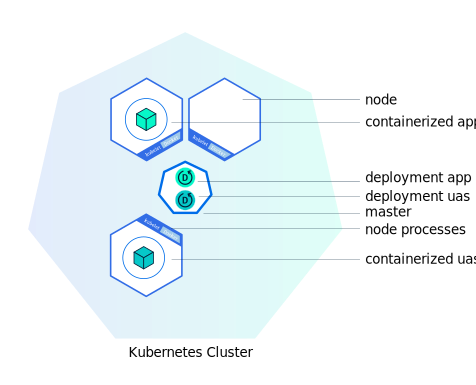
\includegraphics[width=.7\columnwidth]{kubernetes-uas}
	\caption{Kubernetes User API Server}
\end{figure}


% %
% METRICS API
% %
\section{Metrics}
\label{sec:kubernetes-metrics}
Understanding how an application behaves when deployed is crucial to scaling the application and providing a reliable service. In a Kubernetes cluster, application performance can be examined at many different levels: containers, pods, services, and whole clusters. As part of Kubernetes we want to provide users with detailed resource usage information about their running applications at all these levels. This will give users deep insights into how their applications are performing and where possible application bottlenecks may be found. In comes Heapster, a project meant to provide a base monitoring platform on Kubernetes.

Heapster is a cluster-wide aggregator of monitoring and event data. It currently supports Kubernetes natively and works on all Kubernetes setups. Heapster runs as a pod in the cluster, similar to how any Kubernetes application would run. The Heapster pod discovers all nodes in the cluster and queries usage information from the nodes’ Kubelets, the on-machine Kubernetes agent. The Kubelet itself fetches the data from cAdvisor. Heapster groups the information by pod along with the relevant labels. This data is then pushed to a configurable backend for storage and visualization. Currently supported backends include InfluxDB (with Grafana for visualization), Google Cloud Monitoring and many others described in more details here. The overall architecture of the service can be seen below:

\begin{figure}	
	\label{fig:kubernetes-monitoring-architecture}
	\centering
	\includegraphics[width=.7\columnwidth]{kubernetes-monitoring-architecture}
	\caption{Kubernetes monitoring architecture leveraging Heapster.}
\end{figure}

cAdvisor is an open source container resource usage and performance analysis agent. It is purpose-built for containers and supports Docker containers natively. In Kubernetes, cAdvisor is integrated into the Kubelet binary. cAdvisor auto-discovers all containers in the machine and collects CPU, memory, filesystem, and network usage statistics. cAdvisor also provides the overall machine usage by analyzing the ‘root’ container on the machine.

On most Kubernetes clusters, cAdvisor exposes a simple UI for on-machine containers on port 4194. Here is a snapshot of part of cAdvisor’s UI that shows the overall machine usage:

%\begin{figure}	
%	\label{fig:kubernetes-cadvisor-ui}
%	\centering
%	\includegraphics[width=.7\columnwidth]{kubernetes-cadvisor-ui}
%	\caption{Interfaces of cAdvisor.}
%\end{figure}

A Grafana setup with InfluxDB is a very popular combination for monitoring in the open source world. InfluxDB exposes an easy to use API to write and fetch time series data. Heapster is setup to use this storage backend by default on most Kubernetes clusters. A detailed setup guide can be found here. InfluxDB and Grafana run in Pods. The pod exposes itself as a Kubernetes service which is how Heapster discovers it.

The Grafana container serves Grafana’s UI which provides an easy to configure dashboard interface. The default dashboard for Kubernetes contains an example dashboard that monitors resource usage of the cluster and the pods inside of it. This dashboard can easily be customized and expanded. Take a look at the storage schema for InfluxDB here.

%\begin{figure}	
%	\label{fig:kubernetes-heapster-ui}
%	\centering
%	\includegraphics[width=.7\columnwidth]{kubernetes-heapster-ui}
%	\caption{Interfaces of Heapster leveraging Grafana.}
%\end{figure}

Starting from Kubernetes 1.8, resource usage metrics, such as container CPU and memory usage, are available in Kubernetes through the Metrics API. These metrics can be either accessed directly by user, for example by using kubectl top command, or used by a controller in the cluster, e.g. Horizontal Pod Autoscaler, to make decisions.

Through the Metrics API you can get the amount of resource currently used by a given node or a given pod. This API doesn’t store the metric values, so it’s not possible for example to get the amount of resources used by a given node 10 minutes ago.

The API no different from any other API:

it is discoverable through the same endpoint as the other Kubernetes APIs under /apis/metrics.k8s.io/ path
it offers the same security, scalability and reliability guarantees
The API is defined in k8s.io/metrics repository. You can find more information about the API there.

Note: The API requires metrics server to be deployed in the cluster. Otherwise it will be not available.

Metrics Server is a cluster-wide aggregator of resource usage data. Starting from Kubernetes 1.8 it’s deployed by default in clusters created by kube-up.sh script as a Deployment object. If you use a different Kubernetes setup mechanism you can deploy it using the provided deployment yamls. It’s supported in Kubernetes 1.7+ (see details below).

Metric server collects metrics from the Summary API, exposed by Kubelet on each node.

Metrics Server registered in the main API server through Kubernetes aggregator, which was introduced in Kubernetes 1.7.

Learn more about the metrics server in the design doc.
\section{Implementation}
\label{sec:implementation}

The bot has been realized as a Maven-based\footnote{it follows the structure of the basic quickstart archetype.} Java\footnote{Oracle Java 1.8} desktop application, packaged into a self-contained\footnote{fat jar encapsulating all external dependencies.} jar with shrunk and obfuscated code (\Cref{sec:concealment}).

Basically, the bot implements the finite state automaton (\Cref{sec:bot}) and the functionalities required for configuration parsing (\Cref{sec:configuration}), commands execution (\Cref{sec:commands}) and logging (\Cref{sec:logging}). All functionalities has been tested carefully against 123 total JUnit tests.

\textcolor{green}{WEB INTERFACE IMPLEMENTATION \lipsum[1]}

Our bot and web user interfaces leverage some of well known technologies. Here we present them, giving an idea about how they have been used in our implementation. The reader may refer to the open source code of the project and the corresponding Javadocs to get into implementation details.

\begin{description}
  \setlength\itemsep{1em}

  \item[QUARTZ] job scheduling framework developed by the Terracotta Inc \cite{quartz-scheduler}.
  It is a widely adopted solution to support process workflow and system management in enterprise applications.
  In our application it is used for the scheduling of attacks and the sleep mode.

  \item[LOG4J2] logging framework developed by the Apache Software Foundation \cite{log4j2}.
  Together with its main competitor, Logback, it is a de facto standard for logging in Java. Tipically it is used as a bunding of SLF4J, that is a widely adopted logging facade.
  In our application, it is used both for console and file logging.

  \item[COMMONS CLI] command line parsing framework developed by the Apache Software Foundation as a part of the bigger Jakarta project\cite{commons-cli}.
  It is a well known solution for argument parsing in CLI based Java applications.

  \item[JACKSON] serialization framework developed by the Fasterxml team \cite{jackson,fasterxml}.
  It supports most of the widespread serialization format, such as JSON, XML, YAML and so on.
  In our application it is used to serialize/deserialize configuration (in YAML) and commands (in JSON).

  \item[LOMBOK] framework of annotations encapsulating boilerplates and simple patterns \cite{lombok}.
  In our application it is used to generate constructors getters/setters toString/hashCode methods. As such a generation is evaluated at compile time, the code of entity classes is considerably reduced.

  \item[BOOTSTRAP] \textcolor{green}{\lipsum[1]}

  \item[JQUERY] \textcolor{green}{\lipsum[1]}

\end{description}


\subsection{Concealment}
\label{sec:concealment}

Since the bot is a malicious software, his first priority is not to be discovered by the victim's system. Just like any malware, bots should be easily distributed, act covertly and evade the health checks of the infected system. Such a concealment can be achieved, in the first instance, by making the code \textit{minimal, efficient and obfuscated}.

Code minimization allows to distribute the bot in a small sized package, which is easy to conceal in an infection vector, easy to trasmit and whose installation on the system goes unnoticed.
Code efficiency allows the bot to act in a minimally invasive way in terms of memory usage, access to local resources, external communications and sub-processes creation.
Code obfuscation allows the bot to evade traditional health checks based on code patterns analysis. As a beneficial side effect, an obfuscation dictionary with short words can assist code minimization.

All of these aspects concerning the bot concealment have been implemented leveraging \textit{Proguard}, an utility for Java bytecode shrinking, optimization and obfuscation developed by the GuardSquare Inc. \cite{proguard}. ProGuard is the most popular optimizer for Java bytecode. It can make Java applications up to 90\% smaller, up to 20\% faster and protected against reverse engineering\cite{guardsquare}. Such great results makes it a widespread solution in the

In our application, Proguard has been embedded into the Maven packaging life-cycle via an ad-hoc plugin \cite{proguard-maven-plugin}. The adopted configuration of Proguard behaviour can be found in \texttt{config.pro}. From the configuration you may notice a conservative approach. The widespread use of reflection, serialization and annotations in the framework the bot code depends on, makes it necessary to limit both the shrinking and the obfuscation of these frameworks. A deeper code inspection on these frameworks would allow a more aggressive approach, thus obtaining a more minimized and obfuscated code. \footnote{Code obfuscation is subjected to a crucial tradeoff, because the excessive or naive code obfuscation may have collateral side effects. The obfuscation of the whole legitimate code may arouse suspicion of a meticolous checks, because only a legitimate program of high industrial value has no dependency on legitimate clear code. On the other hand, legitimate code letting guess actions of malicious program should never left clear.}.


\subsection{Logging}
\label{sec:logging}

Our bot logs both on console and file adopting a logging discipline that depends on the chosen execution mode.
Console logging prints events on the standard output\footnote{standard error is never used, neither in case of warnings nor errors.}.
File logging deals with two types of events: it appends received commands in \texttt{data/logs/commands.log} and attacks in \texttt{data/logs/attacks.log}. These two files are emptied every time the bot is started.

A general console log message has the following pattern

\begin{verbatim}
  [timestamp] [tread-name] [log-level] [class] [method] - [message]
\end{verbatim}

A file log message about commands has the following pattern

\begin{verbatim}
  [timestamp] Received [COMMAND] with [PARAMS] from CC at [CC-RESOURCE]
\end{verbatim}

A file log message about attacks has the following pattern

\begin{verbatim}
  [timestamp] Launching HTTP attack: [HTTP-METHOD] {TARGET} ([ITER]/[ITERS])
              with proxy [ADDR:PORT] and [HTTP-REQUEST-PROPS]
\end{verbatim}


The \texttt{default} mode prints in console the strictly relevant output and produces log files. The \texttt{trace} mode prints in console a detailed tracing output and produces log files. The \texttt{silent} mode does neither print anything in console nor produce any log file.
To run the program in one of these modes, specify the corresponding option, as indicated in \Cref{sec:helper}.

\chapter{Evaluation}
\label{chp:evaluation}


% %
% HEADER
% %
%\lipsum[1]
Insert the chapter introduction here.


% %
% ENVIRONMENT
% %
\section{Environment}
\label{sec:evaluation-environment}
Describe the environments where the simulator is executed.


% %
% WORKLOAD
% %
\section{Workloads}
\label{sec:evaluation-workloads}
Describes the different workloads given in input to the simulator.

% %
% EXPERIMENTS
% %
\section{Results}
\label{sec:evaluation-results}
Describe every experiment that has been conducted with the respective results.
\section{Conclusions}
\label{sec:conclusions}

%%
% SUMMARY
%%
In this work we propose a next-event simulator for a two-layer Cloud system with off-loading policy on class-partitioned workload, whose random components leverage a multi-stream Lehmer pseudo-random number generator.

%%
% CONCLUSIONS
%%
We may conclude that (i) our simulator returns experimental results that are consistent with the theoretical ones, (ii) the system can achieve the steady-state (iii) the choice of the threshold $S$ is critical for system performances and (iv) the adopted preemption policy allows to balance response time for classes of tasks with different service rates. 

%%
% IMPROVEMENTS
%%
Although our results are pretty satisfactory, the proposed solutions could certainly be improved and be subjected to a more in-depth analysis.
%
From an implementation point of view, the proposed solution should be ported from Python to C and leverage multi-threading to achieve better performances, e.g. to speed-up the algorithms to find suitable multipliers for modulus in 64-bit architectures and make faster simulations.
%
From an analysis point of view, the proposed random number generator should be tested more extensively. For example, we may (i) take into account more tests of randomness (ii) use a pseudo-random number generator with a 64-bit modulus and less number of streams.
%
Finally, the simulation model should be extended in order to 
(i) study the influence of different server selection policies, e.g. equity-selection, and 
(ii) achieve more performance evaluation goals, such as forecasting with respect to the variation of the arrival processes.

\appendix
\section{Usage}
\label{sec:usage}

The program can be run as a java project inside an IDE, as a Maven project or as a self-contained Jar.
In a real scenario, the program would be delivered via an infected file as a self-contained Jar with minimized and obfuscated code \cite{anderson2008security}. Therefore, here, we will show only this compilation and execution method.
The reader may refer to the \texttt{README} file for details on other compilation and execution methods.

In the following, we assume that the execution environment is provided with JDK SE 8 (downloadable from \cite{jdk}) and Maven 3 (downloadable from \cite{maven}). We also assume that both the Jar execution and the path of the files referenced in the configuration do not require any root rights.

\subsection{Compilation}
\label{sec:compilation}

The bot is compiled into a self-contained Jar using the Maven packaging procedure, running the command:

\begin{verbatim}
  $[bot-dir]> mvn package -P optimize,skip-tests
\end{verbatim}

The previous command executes the packaging using both the profile \texttt{optimize} and \texttt{skip-tests}.

Since the bot code should always be optimized (i.e. minimized and obfuscated), we recommend providing this stage, activating the \texttt{optimize} profile. The code optimization is realized by running Proguard in the background (downloadable from \cite{proguard}) and may slow down the compilation. If the execution environment doesn't provide it, or you don't require code optimization, or you want to speed up the compilation, simply omit the corresponding profile.

Since the project involves more than one hundred JUnit tests, we recommend skipping them to speed up compilation, activating the \texttt{skip-tests} profile. If you considered necessary to perform tests, simply omit the corresponding profile.

The compilation produces a jar file \texttt{botnet-1.0-optimized.jar} in the \texttt{target} folder. Since it is self contained, it can be run in any system directory. In the following, we refer to this jar with the shorter name \texttt{botnet.jar}.


\subsection{Execution}
\label{sec:execution}

The program provides the user with three execution mode: \texttt{default}, \texttt{trace} and \texttt{silent}, which are distinguished by the adopted logging discipline. The \texttt{default} mode prints in console the strictly relevant output and produces log files. The \texttt{trace} mode prints in console a detailed tracing output and produces log files. The \texttt{silent} mode does neither print anything in console nor produce any log file.
To run the program in one of these modes, specify the corresponding option, as indicated in \Cref{sec:helper}.
For more details about logging, please refer to \Cref{sec:bot-implementation}.

The program behaviour can be customized providing a custom YAML configuration file. If no configuration is specified, the program runs with default configuration. To run the program with custom configuration, specify the corresponding configuration, as indicated in \Cref{sec:helper}. For more details about configuration, please refer to \Cref{sec:bot-configuration}.

To run the program with default configuration and default execution mode, run the command:

\begin{verbatim}
  $> java -jar botnet.jar
\end{verbatim}

To run the program in \texttt{trace} execution mode, run the command:

\begin{verbatim}
  $> java -jar botnet.jar --trace
\end{verbatim}

To run the program in \texttt{silent} execution mode, run the command:

\begin{verbatim}
  $> java -jar botnet.jar --silent
\end{verbatim}

To run the program with custom configuration, run the command:

\begin{verbatim}
  $> java -jar botnet.jar --config <CONFIG-FILE>
\end{verbatim}

\subsection{The program helper}
\label{sec:helper}

The reader may refer to the program CLI helper for the options usage. We show here the helper output for reader's convenience.

\begin{verbatim}
  BOTNET version 1.0-SNAPSHOT
  Team: ACM Rome Tor Vergata (http://acm.uniroma2.it)

  A botnet showcase.
  Coursework in Computer Security 2015/2016

  usage: BOTNET [-c <CONFIG-FILE>] [-h] [-s] [-t] [-v]
   -c,--config <CONFIG-FILE>   Custom configuration.
   -h,--help                 Show app helper.
   -s,--silent               Activate silent mode.
   -t,--trace                Activate trace mode.
   -v,--version              Show app version.
\end{verbatim}

\subsection{Sample executions}
\label{sec:sample-executions}

\textcolor{blue}{\lipsum[1]}

\begin{verbatim}
$> java -jar botnet -config config-custom.yaml -trace
\end{verbatim}

\textcolor{blue}{\lipsum[1]}

%        plain   normal style - listed in ABC order and labeled numerically
%        unsrt   same as plain except entries appear in order of citation
%        alpha   same as plain except entry labels are used
%        abbrv   same as plain except uses abbreviations for first names,
%                month names, and journal names
\begin{singlespace}
\bibliographystyle{apalike}
\bibliography{bib/main}
\end{singlespace}

\chapter*{Notes}
\label{chp:notes}

\section*{A review of auto-scaling techniques for elastic applications in cloud environments}
\label{sec:lorido2014review}

Notes taken from \cite{lorido2014review}.

Cloud computing environments allow customers to dynamically scale their applications.


\section*{Borg, omega, and kubernetes}
\label{sec:burns2016borg}

Notes taken from \cite{burns2016borg}.


\section*{Reinforcement learning: An introduction}
\label{sec:sutton1998reinforcement}

Notes taken from \cite{sutton1998reinforcement}.

\end{document}
